% !TEX root = Projektdokumentation.tex

\newglossaryentry{XML External Entitiy} {name={XML External Entitiy-Attacke},description={}} % TODO Erklären

\section{Verbesserung der bestehenden Lösung}

\subsection{Frage-Template}
Die Möglichkeit, Fragen offline zu erstellen und anschliessend hochzuladen, bestand bereits. Unterstützt wurde die Erfassung von Singechoice und Multiplechoice-Fragen. Dazu konnten Fragen in eine CSV-Datei geschrieben werden. Alle korrekten Antworten wurden mit einem Asterisk (Stern-Zeichen) versehen. Eine Multiplechoice-Frage lag vor, wenn mehr als eine Antwort mit einem Asterisk versehen war.

In dieser Arbeit wurde das CSV-Template durch ein Excel-Template abgelöst. Die Gründe dazu sind die folgenden:
\begin{itemize}
	\item Die Regeln für das Erstellen waren einem kleinen Personenkreis bekannt. Sie wurden auf der Webseite nicht beschrieben. Damit die Funktion aber Verbreitung findet, muss die Vorgehensweise öffentlich zugänglich sein.
	
	Es wurde entschieden, ein Excel-Template zum Download auf der Webseite anzubieten. Darin sind alle relevanten Informationen für die Erstellung vorhanden.
	
	\item Werden die Fragen in Excel erstellt und anschliessend daraus eine CSV-Datei generiert, so hat man die Wahl zwischen 3 verschiedenen CSV-Varianten.
	
	Der Excel-Import hingegen unterstützt alle Excel-Dateien mit der Endung .xlsx. Dieses Format ist ab Excel 2007 das Standardformat und daher weit verbreitet.
	\cite{microsoft2016}
	
	\item Das CSV-Template war auf Singlechoice und Multiplechoice - Fragen beschränkt.
	
	Da neue Fragetypen unterstützt werden sollten, wurde eine neue Struktur mittels Excel erarbeitet. Um den Ersteller zu Unterstützen wurde mit Farben und weiteren Funktionen gearbeitet, welche durch CSV nicht unterstützt werden.
\end{itemize}

Ein Beispiel des ursprünglichen Formats sowie des neuen Excel-Templates ist im Anhang, im Kapitel 19 Details zur Lösungsfindung, ersichtlich.

Der neue Template-Import wurde mit PHPExcel \cite{phpexcel} umgesetzt. Diese PHP-Library war bereits im Projekt eingebunden und wird dazu verwendet, die Rangliste aller Teilnehmenden eines Quiz zu Exportieren. Die neue Logik befindet sich hauptsächlich in der neu erstellen Datei 'importExcel.php'.

Bei PHPExcel gab es bis zur Version 1.7.9 eine \gls{XML External Entitiy} - \gls{Vulnerability}. Dadurch war es Remote-Angreifern möglich, beliebige Dateien auf dem Server zu lesen oder eine Denial-of-Service - Attacke durchzuführen. \cite{cvedetails_phpexcel} %TODO Remote und Denial-of-Service erklären
Da bei MobileQuiz allerdings die Version 1.8.0 verwendet wird, ist dies nicht mehr möglich. Es wurde mit dem Wissen von InfSi3 versucht eine solche Attacke durchzuführen, was ebenfalls zum Ergebnis führte, dass diese Sicherheitslücke nicht mehr vorhanden ist. %TODO InfSi3 erklären

\section{Neuerungen}

\subsection{Fragen mit Bildern}

\subsubsection{Hochladen und Entfernen eines Bildes}
Bei jedem Fragetyp ist es neu möglich ein Bild zu hinterlegen. Die Funktion des Bild-Uploads auf den Server bestand bereits, wurde aber erweitert.
\\
\\
Beim Hochladen des Bildes wurde zuvor eine Fehlermeldung ausgegeben, wenn ein Bild eine Grösse von über 20 Megabyte überstieg. Diese Limite wurde herabgesetzt, weil ein Bild von dieser Grösse lange benötigt, bis es heruntergeladen werden kann. Unten ist ein Vergleich von Downloadzeiten aufgeführt, bei verschiedenen Dateigrössen. Die Downloadgeschwindigkeit ist die durchschnittliche Downloadgeschwindigkeit der Swisscom-Kunden, welche anhand von Speedtests der cnlab AG \cite{cnlab_speedtest} ermittelt wurde. Es wurden die Swisscom-Kunden gewählt, weil die Anzahl der User dort am grössten war. \\

\begin{tabular}{|c|c|c|}
	\hline 
	Dateigrösse & Downloadgeschwindigkeit & Benötigte Zeit \\ 
	\hline 
	20 MB & 33,1 Mbit/s & 4,8 s \\ 
	\hline 
	5 MB & 33,1 Mbit/s & 1,2 s \\ 
	\hline 
	800 KB & 33,1 Mbit/s & 0,2 s \\ 
	\hline 
\end{tabular}\\

Falls ein Bild nun 800 Kilobyte übersteigt, so wird es so lange komprimiert, bis seine Dateigrösse darunterliegt. Dies wird durch die PHP-Funktion 'imagecopyresampled' erreicht. Als Code-Vorlage diente das Beispiel von www.williseiler.ch \cite{willis_php}. \\

Weiter gibt es Grössenbeschränkungen von Apache selbst \cite{stackoverflow_largeFilePHP}. Im File 'php.ini' können folgende drei Werte definiert werden:
\begin{itemize}
	\item upload\_max\_filesize: Legt die maximale Dateigrösse für eine Upload-Datei fest. Der Standardwert liegt bei 2 MB.
	\item post\_max\_size: Legt die maximale Grösse aller POST-Daten zusammen fest. Der Standardwert liegt bei 8 MB.
	\item max\_file\_uploads: Legt die maximale Anzahl aller Dateien fest, welche auf einmal hochgeladen werden können. Der Standardwert liegt bei 20 Dateien.
\end{itemize}

Werden via Excel-Template 10 Fragen mit je einem Bild à 1 Megabyte hochgeladen, so ist dies mit der Standardkonfiguration nicht möglich. Diese wurde deshalb folgendermassen angepasst:
\begin{itemize}
	\item upload\_max\_filesize: Neu 5 MB. Grössere Dateien benötigen zu lange für den Upload, allerdings soll der Benutzer nicht nur auf kleine Grössen beschränkt sein. Deshalb wurde von der 2MB-Standardgrösse abgewichen.
	\item post\_max\_size: Neu 25 MB. Bei dieser Grösse beträgt die Uploadzeit bei einer Geschwindigkeit von 15 Mbit/s 13 Sekunden. Dies ist die Durchschnittliche Uploadgeschwindigkeit von Swisscom-Kunden, welche beim Speedtest der cnlab AG \cite{cnlab_speedtest} erreicht wurde. Diese Messungen umfassen jedoch auch Mobile-Messungen mit Smartphones. Da die Uploads der Frage-Templates aber eher von Computern und Laptops erfolgen, welche dank LAN und WLAN eine höhere Uploadgeschwindigkeit aufweisen, ist diese Uploadzeit eher geringer. Der Benutzer sollte sich zudem bewusst sein, dass der Upload bei so vielen Dateien einige Zeit in Anspruch nimmt.
	Auf der anderen Seite soll der Benutzer aber auch nicht eingeschränkt werden. Es soll möglich sein, gleichzeitig 20 Fragen mit Bildern à 1 MB sowie 1 Frage mit einem grösseren Bild plus Excel-Template hochzuladen.
	\item max\_file\_uploads: Neu 25 Dateien. Der Standard-Wert wird nur leicht angehoben, da es möglich sein soll 20 Fragen mit Bildern gleichzeitig zu erstellen. Damit würde das Maximum von 20 Dateien nicht ausreichen.
\end{itemize}

Beim Upload wird das mit folgendem Dateinahmen im Ordner 'uploadedImages' abgelegt: 'question\_Datum(Tag\_Monat\_Jahr\_Stunde\_Minute\_Sekunde\_\_SessionId.Dateityp'.
\\
\\
Das Excel-Template für die Frage-Erstellung wurde ebenfalls erweitert, dass auch Fragen mit Bildern erstellt werden können. Dazu wurde eine neue Spalte eingefügt, bei welcher man den Bildnamen inklusive Endung einträgt. Die Bilder müssen sich dabei im gleichen Ordner wie das Template befinden. Anschliessend wird der gesamte Ordner hochgeladen.

Es war dabei nicht möglich, nur die Excel-Datei alleine hochzuladen und anschliessend die Bilder selbstständig zu holen. Dies wäre bezüglich der Sicherheit höchst bedenklich.
\\
\\
Wird eine Frage gelöscht, so wird nebst dem Datenbankeintrag auch das Bild vom Server entfernt.


\subsubsection{Änderungen am Server}
\textbf{Wichtig:} 
Für den Server-Upload müssen die folgenden zwei Dinge gegeben sein:
\begin{itemize}
	\item Die PHP-Library 'GD' muss für die Bildverarbeitung installiert sein. Ob dies der Falls ist kann mittels PHPInfo() oder nachfolgendem Code festgestellt werden. \cite{zoopable.com} Sollte 'GD' nicht installiert sein, so ist unten ebenfalls der Installationsbefehl aufgeführt. \cite{askubuntu.com_php_extension}
\end{itemize}
\begin{lstlisting}
<?php
if (extension_loaded('gd') && function_exists('gd_info')) {
echo "PHP GD library is installed on your web server";
}
else {
echo "PHP GD library is NOT installed on your web server";
}
?>

sudo apt-get install php5.6-gd
\end{lstlisting}

\begin{itemize}
	\item Die Childprozesse des Apache-Servers, welche die Anfragen beantworten, benötigen Schreibrechte auf den Upload-Ordner. Ob dies gegeben ist, kann mittels folgendem Befehl überprüft und geändert werden. \cite{askubuntu.com_permissions} 
\end{itemize}
\begin{lstlisting}
ps -ef | grep apache | grep -v grep
\end{lstlisting}

\begin{lstlisting}
root      5001     1  0 07:21 ?    00:00:00 /usr/sbin/apache2 -k start
www-data  5021  5001  0 07:21 ?    00:00:00 /usr/sbin/apache2 -k start
www-data  5022  5001  0 07:21 ?    00:00:00 /usr/sbin/apache2 -k start
www-data  5023  5001  0 07:21 ?    00:00:00 /usr/sbin/apache2 -k start
\end{lstlisting}

Ist die Ausgabe wie oben ersichtlich, so werden die Anfragen von Prozessen der Benutzergruppe 'www-data' beantwortet. Die Schreibrechte an diese Gruppe können wie folgt vergeben werden:
\begin{lstlisting}
chgrp www-data /path/to/mydir
chmod g+w /path/to/mydir
\end{lstlisting}




\subsubsection{Anzeige eines Bildes}
Das Bild sollte beim Anzeigen der Frage gross genug dargestellt werden. Auf dem Computer war dies kein Problem, da ein Browserfenster genug Platz dazu bot, bei einem Smartphone hingegen war dieser beschränkt. Deshalb wurde die Anzeige so umgesetzt, dass das Bild beim Klick darauf auf dem ganzen Bildschirm dargestellt wird. Dies wurde mit Photoswipe \cite{photoswipe} umgesetzt, welches von GitHub \cite{github_photoswipe} bezogen wurde. Photoswipe ist eine JavaScript-Library, welche es ermöglicht, Bildgalerien auf Websites darzustellen. Sie unterstützt unter anderem Touch-Gesten und Zoom. So ist es kein Problem, ein Bild mit vielen Details darzustellen.

Nachfolgend ist zu sehen, wie eine Frage mit Bild in verschieden Situationen angezeigt wird.

\begin{figure}[H]
	\centering
	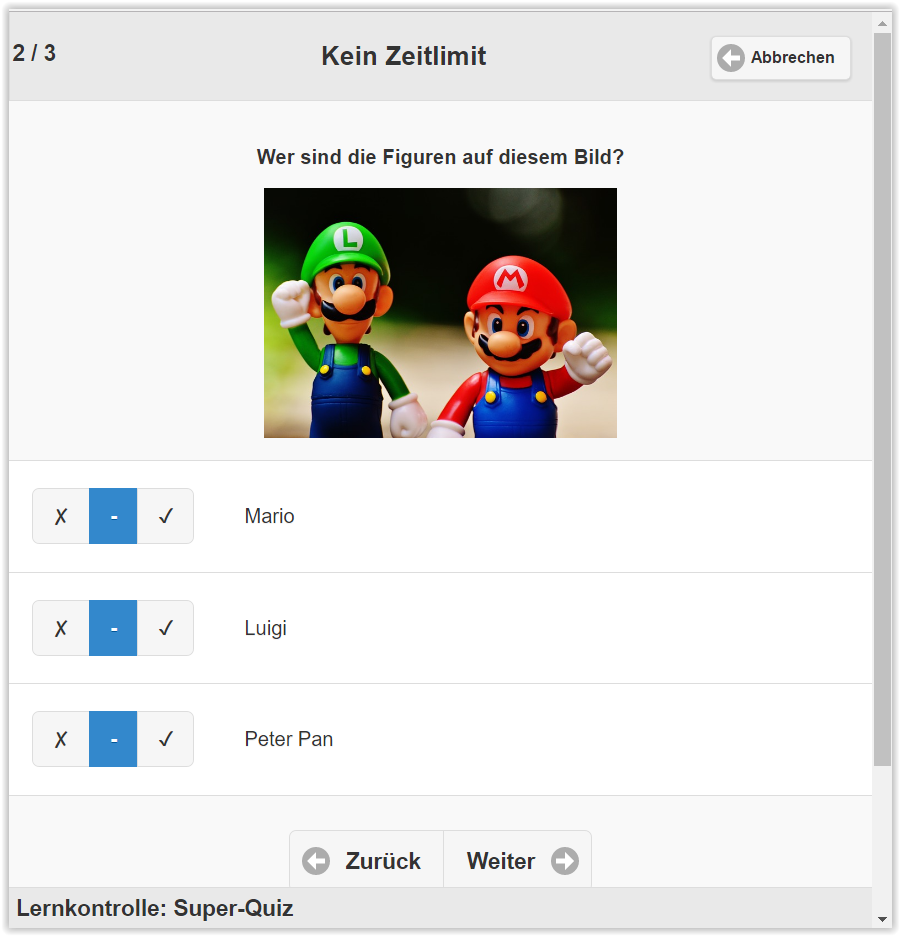
\includegraphics[width=0.75\textwidth]{Images/Frage-Bild_Anzeige_PC.PNG}
	\caption{Anzeige des Frage-Bildes am Computer}
	Quelle: Mobilequiz.ch / Fragebild: https://pixabay.com/de/mario-luigi-figuren-lustig-bunt-1558012/
\end{figure}

\begin{figure}[H]
	\centering
	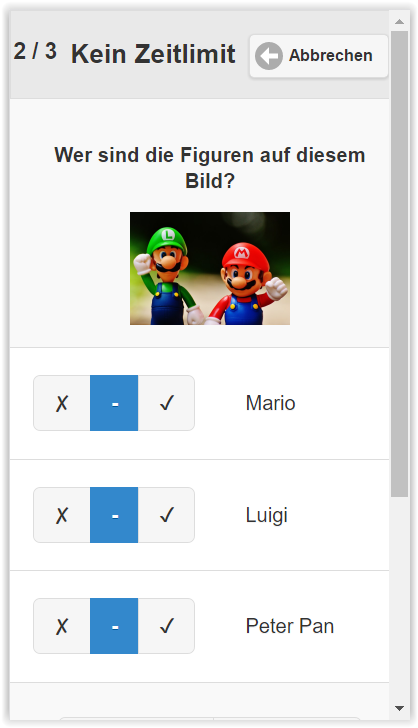
\includegraphics[width=0.3\textwidth]{Images/Frage-Bild_Anzeige_Mobile.PNG}
	\caption{Anzeige des Frage-Bildes auf dem Smartphone}
	Quelle: Mobilequiz.ch / Fragebild: https://pixabay.com/de/mario-luigi-figuren-lustig-bunt-1558012/
\end{figure}

\begin{figure}[H]
	\centering
	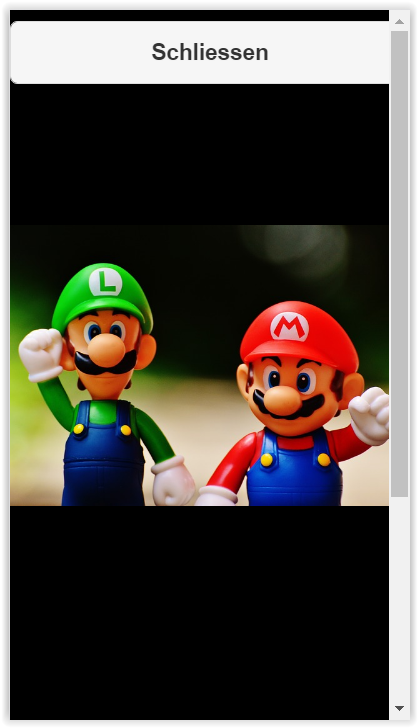
\includegraphics[width=0.3\textwidth]{Images/Frage-Bild_Anzeige_Mobile_Full.PNG}
	\caption{Fullscreen-Anzeige des Frage-Bildes auf dem Smartphone}
	Quelle: Mobilequiz.ch / Fragebild: https://pixabay.com/de/mario-luigi-figuren-lustig-bunt-1558012/
\end{figure}


Weiter wurde die Generierung des PDF-Aufgabenblattes und Lösungsblattes ergänzt, damit auch dort die Bilder angezeigt werden. Hat man unterwegs kein Internet, so kann man sich die Fragen damit auch vorgängig herunterladen und im Zug anschauen.


